\documentclass[12pt]{report}
\usepackage[utf8]{inputenc}
\usepackage{amsmath}
\usepackage{graphicx}
\usepackage{subcaption}
\usepackage{caption}
\usepackage{tabls}
\usepackage{afterpage}
\usepackage{epsf}
\usepackage{color}
\usepackage{algorithm}
\usepackage[noend]{algpseudocode}
\usepackage{lmodern}
\usepackage{lipsum}
\usepackage{todonotes}
\usepackage[titletoc]{appendix}
% necessary commands
\newcommand{\chig}{\chi_\rg}
\newcommand{\sn}{S$_N$}
\newcommand{\varphigp}{\varphi_{\rg'}}
\newcommand{\varphig}{\varphi_\rg}
\newcommand{\need}[1]{\textcolor{red}{#1}}
\newcommand{\md}{\mathcal{D}}
\newcommand{\pd}{\partial\md}
\newcommand{\mm}[1]{\mathrm{#1}}
\newcommand{\rg}{\mm{g}}
\newcommand{\mrm}{\mm{m}}
\newcommand{\rgp}{{\rg'}}

\usepackage{geometry}
\geometry{margin=1in}

\title{A Two-Grid, Nonlinear Diffusion Acceleration Method for the $S_N$ Equations with Neutron Upscattering}
\author{Marissa Ramirez Zweiger }
\date{July 27th, 2018}


\begin{document}
\pagestyle{empty}
\begin{center}
A Two-Grid, Nonlinear Diffusion Acceleration Method  \\ 
for the $S_N$ Equations with Neutron Upscattering \\
\vspace{20mm}
by \\
\vspace{5mm}
Marissa Ramirez Zweiger \\ 
\vspace{20mm}
A thesis submitted in partial
satisfaction of the \\
\vspace{5mm}
requirements for the degree of \\
\vspace{5mm}
Master of Science \\
\vspace{5mm}
in \\
\vspace{5mm}
Nuclear Engineering \\
\vspace{5mm}
in the \\
\vspace{5mm}
Graduate Division \\
\vspace{5mm}
of the \\
\vspace{5mm}
University of California, Berkeley \\
\vspace{20mm}
Committee in charge: \\
\vspace{5mm}
Professor Rachel Slaybaugh, Chair \\
Professor Phillip Colella \\
Professor Massimiliano Fratoni \\
\vspace{5mm}
Summer 2018
\end{center}



\renewcommand{\abstractname}{Acknowledgements}
\begin{abstract}
\pagenumbering{roman}
\thispagestyle{plain}
I would like to acknowledge my advisers, Dr. Rachel Slaybaugh and Dr. Phillip Colella, as well as my third committee member, Dr. Max Fratoni, for their guidance. This work would not have been possible without the mentorship of Dr. Weixiong Zheng - Thank you. I am also particularly appreciative of my colleagues, Joshua Rehak and Mario Ortega who were always willing to talk through concepts and let me bounce ideas off of them. 

Most of all, my gratitude goes to my family. Thank you to my mother, Andrea Ramirez, who has always been a constant source of support and to my partner in all things, Marcell Vazquez-Chanlatte, for always having handy the things I've needed most: useful python tricks, a blackboard, and a warm cup of tea. 
\end{abstract}

\tableofcontents

\chapter{Introduction}
\setcounter{page}{2}
\pagenumbering{arabic}
\label{sec:intro}
The field of computational neutronics, computationally solving the Boltzmann Transport equation applied to neutrons (transport equation), is generally concerned with modeling neutrons in a nuclear system. These systems include nuclear reactors or shielding problems where there exists a fixed source of neutrons. The materials used in these systems have a variety of properties, including how they effect the energy of the neutron. Many materials that are commonly used in nuclear applications, particularly those containing hydrogen, exhibit significant upscattering, where lower energy neutrons are ``bounced" to higher energies. The details of scattering can dramatically impact which numerical methods to choose, particularly when solving the transport equation deterministically \cite{park-nda}. 

Hydrogen based materials, such as graphite or heavy water, are often used as moderators in nuclear reactors. These problems, with upscattering and little leakage or absorption, are traditionally very computationally expensive ~\cite{morel-upscat}. A significant cause of the large computational cost comes from the number of iterations needed to converge the problem. The steady-state transport equation is dependent on space, angle, and energy. It is often solved via a series of nested iterations. The various iteration methods and how they are used with each other are described in detail in Ch. \ref{sec:iterative}. In this work I target two layers of iteration, the ``within-group" and the ``multi-group" iterations, attempting to reduce the total number of iterations needed and thus the run time. The first method I use, Nonlinear Diffusion Acceleration (NDA), happens in the within-group, or source, iteration, where angle and energy are fixed. The second method, which to our knowledge has never been applied to NDA, targets the multigroup solver, Gauss-Seidel. Gauss-Seidel is one of the most commonly-used methods for iterating over energy groups. It is guaranteed to converge; however, in problems with significant upscattering, the time it takes to reach convergence can become arbitrarily slow \cite{evans-upscat}, which makes it a good candidate for acceleration. 

To accelerate the Gauss-Seidel convergence with upscattering, an energy two-grid (TG) acceleration scheme was first developed to approximate iteration error by solving a one-group diffusion-like equation with artificial material properties generated by using the scattering eigen-spectrum \cite{morel-upscat}. Later, a transport TG (TTG) method was developed that approximates the energy error using a consistent \sn\ solver in multi-D \cite{evans-upscat}. Both of these were developed for use with traditional source iteration, and to our knowledge have not yet been extended for use with NDA. Inspired by the previous studies, I derive a TG scheme for the NDA equation with Gauss-Seidel iteration.


\section{The Boltzmann Transport Equation}
The angular neutron flux of a reactor, $\psi$ can be found by solving the steady state Boltzmann Transport equation,

\begin{equation}
\begin{split}
  [\hat{\Omega} \cdot \nabla + &\Sigma_t(\vec{r}, E)]\psi(\vec{r}, \hat{\Omega}, E) = \frac{\chi(E)}{4\pi} \int_0^\infty dE' \nu \Sigma_{f}(\vec{r}, E') \int_{4\pi} d\hat{\Omega}'\psi(\vec{r}, \hat{\Omega}', E') \\   &+ \int_0^\infty dE' \int_{4\pi} d\hat{\Omega}' \Sigma_s(\vec{r}, E' \rightarrow E, \hat{\Omega}' \cdot \hat{\Omega})\psi(\vec{r}, \hat{\Omega}', E') + Q(\vec{r}, \hat{\Omega}, E)   \:,
\end{split}
\label{eq:transport}
\end{equation}

where $\hat{\Omega}$ represents the angle; $\vec{r}$, the position vector; $E$, the energy; $\Sigma_t$, the total macroscopic cross-section; $\Sigma_f$, the macroscopic fission cross-section; $\Sigma_s$, the macroscopic scattering cross section; $\chi$, the energy distribution with which neutrons are born; $\nu$, the average number of neutrons per fission; and $Q$, an external source.  


In this work, I apply an incident boundary condition, where for $\hat{n} \cdot \hat{\Omega} < 0$, with $\hat{n}$ being the outward normal on the boundary $\partial \mathcal{D}$,
\begin{equation}
    \psi(\vec{r}, \hat{\Omega}, E) = \psi^{inc}(\vec{r}, \hat{\Omega}, E), \hspace{5mm} \vec{r} \in \partial \mathcal{D}\:,
\end{equation}
though other boundary conditions such as reflecting, periodic, and vacuum are valid.

\subsection{Fixed Source Form of the Transport Equation}
There are are several forms of the transport equation that are of interest in the field of nuclear energy. In this work, I present all methods in fixed-source form; however, they can all be easily extended to $k$-eigenvalue form for criticality calculations. 

To write Eqn.~\eqref{eq:transport} in a fixed source form, drop the fission term and retain the source, $Q$. If there is fission in the system, fission neutrons can be included in the source term. I use the same boundary conditions as above. 
%
\begin{equation}
\begin{split}
 [\hat{\Omega} \cdot \nabla + \Sigma(\vec{r}, E)]\psi(\vec{r}, \hat{\Omega}, E) &= \\ \int_0^\infty dE' &\int_{4\pi} d\hat{\Omega}' \Sigma_s(\vec{r}, E' \rightarrow E, \hat{\Omega}' \cdot \hat{\Omega})\psi(\vec{r}, \hat{\Omega}', E')  + Q(\vec{r}, \hat{\Omega}, E)
\end{split}
 \label{eq:transport_fixed_source}
\end{equation}



\section{Space-Angle Approximations of Interest}
There are many simplifications and approximations that can be made to facilitate the solution of the transport equation. In this work, scattering and fixed sources are assumed to be isotropic, which gives the following form
%
\begin{equation}
[\hat{\Omega} \cdot \nabla + \Sigma_t(\vec{r}, E)] \psi(\vec{r}, \hat{\Omega}, E) =   \int_0^\infty \frac{1}{4\pi} \Sigma_s(\vec{r}, E' \rightarrow E)  dE' \int_{4\pi} d\hat{\Omega}'\psi(\vec{r}, \hat{\Omega}', E')  + \frac{1}{4\pi}Q(\vec{r}, \hat{\Omega}, E) .
 \label{eq:transport_isotropic_scattering}
\end{equation}

This equation gives the angular flux. To find the scalar flux, $\phi$, which is often the quantity desired in practice as it is used to give the reactions rates needed for engineering solutions, one must integrate over all directions

\begin{equation}
  \phi(\vec{r}, E) = \int_{4\pi} \phi(\vec{r}, \hat{\Omega}, E) d \hat{\Omega}\:.
\end{equation}


\subsection{The Diffusion Equation}
To simplify even further, I employ a commonly-used approximation, the one-group diffusion equation. To derive the diffusion equation, consider the neutron balance within an infinitesimal volume centered at a point, $r$. For simplicity of notation, I will present this derivation assuming all neutrons have the same energy. Under steady state conditions, neutron conservation requires
%
\begin{equation}
    \textit{net streaming} + \textit{neutrons absorbed} = \textit{source neutrons emitted}.
\end{equation}

The net streaming is described as the rate of the current, $\vec{J} = \int_{4\pi} \vec{\Omega}\psi$, in all directions; the neutrons absorbed is the absorption cross section times the scalar flux, $\Sigma_a\phi$; and the source neutrons are represented by the source variable, $Q$. This gives the neutron continuity equation

\begin{equation}
\nabla\cdot \vec{J}(\vec{r}) + \Sigma_a(\vec{r})\phi(\vec{r}) = Q(\vec{r})\:.
\end{equation}

Using Fick's Law, which relates the current to the flux, $\vec{J}(\vec{r}) = -D(\vec{r})\nabla\phi(\vec{r})$ where $D = 1/3\Sigma_t$, leads to the diffusion approximation

\begin{equation}
\begin{split}
 - \nabla \cdot D(\vec{r})\nabla\phi(\vec{r}) &+ \Sigma_a \phi(\vec{r}) = Q(\vec{r})\:.
\end{split}
\label{eq:diffusion_fixed_source}
\end{equation}

The diffusion equation is much easier to solve than the transport equation because it is not dependent on angle. However, because of the assumptions made in the Fick's Law approximation, it is not valid near boundaries where material properties change dramatically, near localized sources, or in strongly absorbing media \cite{lewis-miller}.

\subsection{Nonlinear Diffusion Acceleration}

This work presents an acceleration to a method known as Nonlinear Diffusion Acceleration (NDA). NDA reformulates the transport equation as a correction to the diffusion equation and uses a two step process to solve. For reference, I repeat the derivation of the low-order NDA equation found in \cite{morel-holo} with small modifications. I assume no fission source and vacuum boundary conditions. Consider the first order, one-group, fixed-source form with isotropic scattering. 


  \begin{equation}
  \hat{\Omega}\cdot \nabla \psi \left(\vec{r}\right)+ \Sigma_{\mm{t}}\left(\vec{r}\right)\psi = \frac{1}{4 \pi} \Sigma_{\mm{s}}\left(\vec{r}\right) \phi\left(\vec{r}\right) + \frac{1}{4 \pi} Q\:.
  \end{equation}
Integrate over all angles to obtain the zeroth moment equation

\begin{equation}
  \nabla \cdot \vec{J} + \Sigma_a\phi  =  Q\:,
  \label{eq:zeroth_moment_1g}
\end{equation}
Now consider the first moment equation:
  \begin{equation}
  \nabla \cdot \overset{\text{\scriptsize$\leftrightarrow$}}{P} + \Sigma_t J = 0\:,
  \end{equation}
where $\nabla \cdot \overset{\text{\scriptsize$\leftrightarrow$}}{P} =  \int_{4\pi} \hat{\Omega} \hat{\Omega} \cdot \nabla \psi$. It can be rewritten as: 

  \begin{equation}
  J= -\frac{1}{\Sigma_t} \nabla \cdot \overset{\text{\scriptsize$\leftrightarrow$}}{P}\:. 
  \end{equation}
  By adding and subtracting the diffusion coefficient multiplied by the gradient of the scalar flux, the first moment equation takes the form of a correction to Fick's Law
  
  \begin{equation}
  J = -D \nabla \phi + D \nabla \phi - \frac{1}{\Sigma_t} \nabla \overset{\text{\scriptsize$\leftrightarrow$}}{P} = -D \nabla \phi - \vec{\textbf{D}} \phi \:,
  \label{eq:fick_corr_1g}
  \end{equation}
  
where $\vec{\textbf{D}}$ is the drift vector
 \begin{equation}
  \vec{\textbf{D}} (\psi) = \frac{\int_{4\pi} [\frac{1}{\Sigma_t} \hat{\Omega} \hat{\Omega}\cdot \nabla \psi] - D \nabla \phi^{ho}}{\phi^{ho}}.
  \label{eq:drift_vector}
  \end{equation} 
$\phi^{ho} = \int_{4\pi} \psi(\hat{\Omega}, \vec{r}) d\hat{\Omega}$ and $\psi$ is the solution of the higher order equation. Substituting Eqn.~\eqref{eq:fick_corr_1g} into Eqn.~\eqref{eq:zeroth_moment_1g} gives the following NDA equation:

  \begin{equation}
  \nabla\cdot(-D \nabla \phi - \vec{\bf D} \phi) + \Sigma_a \phi = Q \:. \label{eq:NDA_1g}
  \end{equation}
  
Because NDA uses the solution from a higher-order calculation to find the the drift vector, it will not give an exact correction. While NDA maintains much of the accuracy of the higher-order equation when compared to diffusion, the two are not exactly equal. 




\subsection{Self-Adjoint Angular Flux}
NDA requires the use of a higher order equation. In this work, I use the Self-Adjoint Angular Flux Form (SAAF) \cite{saaf}. Discretizing the traditional transport equation Eqn.~\eqref{eq:transport_isotropic_scattering} in space, particularly using the finite element method presents a number of challenges \cite{saaf}. A finite element spatial discretization is generally favorable as it produces as symmetric positive-definite (SPD) linear system \cite{zheng-siam}. SPD systems can be solved using a number of well-studied, robust solution techniques \cite{Shewchuck1994}. In order to make use of these properties,  the standard transport equation must be rearranged into a form that is more computationally friendly.

The Self-Adjoint Angular Flux equation is given as

\begin{equation}
    - \vec{\Omega} \cdot \nabla \frac{1}{\Sigma_t}\vec{\Omega} \cdot \nabla \psi + \Sigma_t \psi = \frac{1}{4\pi}[\Sigma_s\phi + Q - \vec{\Omega} \cdot \nabla \frac{(\Sigma_s\phi + Q)}{\Sigma_t}]\:.
    \label{eq:SAAF}
\end{equation}


\subsection{Coupling NDA and SAAF}
NDA and SAAF work together as an acceleration to the source iteration process. Source iteration is a method by which the scalar flux on the right hand side of Eqn.~\eqref{eq:transport_fixed_source} is fixed, so that the equation may be solved with a linear solver. At each iteration, the result of $\phi$ at the previous iteration is used as the guess, until the solutions converge. NDA accelerates source iteration by using a higher order equation to create a correction to the diffusion equation. In this work, I use SAAF as the higher order equation. Below I outline how they work together, using $l$ as the iteration index.

\begin{enumerate}
    \item Intitialize system, by setting $\vec{\textbf{D}}$ to 0 and solving Eqn.~\eqref{eq:NDA_1g} to get $\phi^0$ 
    \item Loop Until Convergence:
        \begin{enumerate}
            \item Solve Eqn.~\eqref{eq:SAAF} for $\psi^l$ using $\phi^{l-1}$ on RHS.
            \item Calculate drift vector, Eqn.~\eqref{eq:drift_vector}, using $\psi^l$
            \item Solve Eqn.~\eqref{eq:NDA_1g} for $\phi^l$
            \item Check $\phi^{l-1}, \phi^l$ for convergence
        \end{enumerate}
    \item Return $\phi$
\end{enumerate}

I am able to replicate the results of \cite{Wang2013}, showing a significant reduction in the number of source iterations necessary when using NDA with SAAF as compared to SAAF alone. However, it is important to note that NDA only accelerates one layer of iteration - the within-group solve. In the following sections I will discuss the acceleration of the multigroup solver.


\section{Methods of Discretization}
The angular flux, $\psi$, is a function of space, angle, and energy. In the solution process, each dimension is discretized. There are several choices that have to be made regarding discretization. In this work, I endeavor to show equation forms that are discretization agnostic as well as showing formulations unique to the particular discretization methods I chose to implement. 

\subsection{Angular Discretization}
 
\begin{figure}[H]
    \centering
    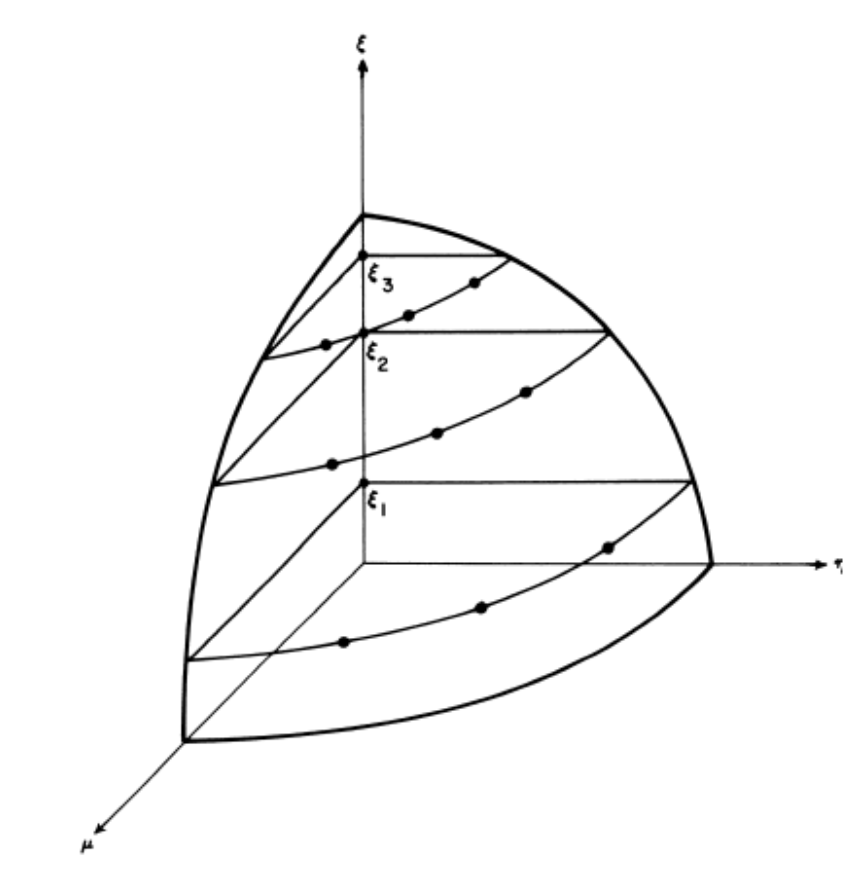
\includegraphics[width=.5\textwidth]{fig/SNPoints.png}
    \caption{Equally-Weighted Gauss-Chebyshev Quadrature Points \cite{Lathrop1965}}
    \label{fig:SN}
\end{figure}
%
Angular discretization of Eqn.~\eqref{eq:transport} is handled via the discrete ordinates ($S_N$) method, a finite-element collocation method \cite{Lathrop1965}. The $S_N$ method uses a quadrature rule, evaluating the equation at number of discrete angles or ``ordinates" and uses corresponding weights to perform a sum that results in integration over the unit sphere. 
For a set of $N$ ordinates with weights $w_n$, a function $f$ integrated over angle as

\begin{equation}
\int \hat{\Omega} f(\hat{\Omega}) d \hat{\Omega} = \sum\limits_{\mrm=1}^{M} w_\mrm f_\mrm.    
\end{equation}

I use a Gauss-Chebyshev angular quadrature set, which can be thought of as a product set, combining a one-dimensional Gaussian Quadrature along the polar angles and an equally-weighted Chebyshev quadrature along the azimuthal angles \cite{jarrel-thesis}. This can be seen in Figure~\ref{fig:SN}. 

The steady-state, one-group $S_N$ transport equation is given as follows,

 \begin{equation}
  \vec{\Omega}_n \cdot \nabla \psi_n \left(\vec{r}\right)+ \Sigma_{\mm{t}}\left(\vec{r}\right)\psi_n = \frac{1}{4 \pi} \Sigma_{\mm{s}}\left(\vec{r}\right) \phi\left(\vec{r}\right) + \frac{1}{4 \pi} Q\left(\vec{r}\right)\:,
  \label{eq:transport-angular}
 \end{equation}
where $n$ is the angular index and $\phi = \sum\limits_{n=1}^N w_n \psi_n$.


\subsection{Energy Discretization}
In the treatment of energy, the full energy spectrum is divided into several energy groups. By convention, the highest energy group is given the index, 1, with the index number going up until it reaches the lowest energy group, $G$. In expanding to multiple energy groups, scattering from one group, $\rg'$, to another, $\rg$, denoted as $\rg' \rightarrow \rg $, must be taken into account. 

The energy discretized, steady-state, transport equation is
%
 \begin{equation}
  \vec{\Omega} \cdot \nabla \psi_\rg \left(\vec{r}\right)+ \Sigma_{\mm{t}, \rg}\left(\vec{r}\right)\psi_\rg = \frac{1}{4 \pi} \sum\limits_{\rg'=1}^{G}\Sigma_{\mm{s}, \rg' \rightarrow \rg}\left(\vec{r}\right) \phi_{\rg'}\left(\vec{r}\right) + \frac{1}{4 \pi} Q_\rg\:.
  \label{eq:transport-energy}
 \end{equation}


\subsection{Spatial Discretization}
In this work, I chose to discretize in two dimensions, assuming uniformity in the third; however, all formulations could be extended to be truly 3D. Spatial discretization methods for the transport equation are usually performed using commonly-known differential equation discretization techniques such as the finite difference, finite volume, or finite element methods. In this work, spatial discretization is performed using the finite element method on triangular elements (described in detail in Appendix \ref{sec:spatial}); however, TG-NDA can be used with any spatial discretization. Here, I give the weak forms of NDA and SAAF for use with the finite element method. Their full derivations can be seen in Appendix \ref{sec:spatial}. 


\subsubsection{Weak Form of Multigroup NDA}

Given a function space $W_\mathcal{D}$, for all $\psi^*$ in $W_\mathcal{D}$, Find $\psi_{\rg} \in W_\mathcal{D}$ such that

\begin{equation}
 \begin{split}
  \left(D_\rg \nabla \psi_\rg^{k+1/2}, \nabla \psi^*\right)_\mathcal{D} + \left(\vec{\bf{D}}_\rg \psi_\rg^{k+1/2} , \nabla \psi^*\right)_\mathcal{D} +  \left(\Sigma_{r,\rg} \varphi_{\rg}^{k+1/2}, \psi^*\right)_\mathcal{D} &=  \\
   \left(\sum\limits_{\substack{\rg'=1}}^\mm{g-1} \Sigma_{\mm{s},\rg' \to\rg}\psi_{\rg}^{k+1/2}, \psi^*\right)_\mathcal{D} + \left(\sum\limits_{\substack{\rg'=\rg+1}}^\mm{G} \Sigma_{\mm{s},\rg' \to\rg}\psi_{\rg}^{k}, \psi^*\right)_\mathcal{D} 
  &+ \left(Q_{\rg}, \psi^*_\rg\right)_\mathcal{D} \:.
 \end{split}
 \label{k1/2-1g}
\end{equation}
%
where the parentheses represent the inner product integrated over a domain $\mathcal{D}$ for a given direction.

\subsubsection{Weak Form of Multigroup SAAF}
Using the boundary condition treatment given in \cite{zheng-thesis}, gives the following weak form:
% Correct this part
Given a function space $W_\mathcal{D}$, for all $\psi^*_{\rg}$ in $W_\mathcal{D}$, Find $\psi_{\rg} \in W_\mathcal{D}$ such that,

\begin{equation}
    \begin{split}
        \left ( \vec{\Omega}\frac{1}{\sigma_{t, \rg}}\vec{\Omega}\cdot \vec{\nabla}\psi_\rg, \vec{\nabla}\psi* \right)_\mathcal{D} -     \left < \hat{n} \cdot \hat{\Omega}\psi_\rg, \psi^* \right>_{\hat{n} \cdot \hat{\Omega} < 0, \Gamma} &+ \left ( \sigma_{t, \rg} \psi_\rg, \psi* \right )_\mathcal{D} = \\
        \left ( q_\rg, \psi* \right)_\mathcal{D} + \left ( \vec{\Omega} \frac{q_\rg}{\sigma_{t, \rg}}, \vec{\nabla}\psi* \right)_\mathcal{D} &- \left < \hat{n} \cdot {\Omega} \psi^{inc}, \psi^* \right>_{\hat{n}, \hat{\Omega} <0, \Gamma} 
    \end{split}
\end{equation}

where $q = \int_{4\pi}(\Sigma_{s, \rg \rightarrow \rg'}\phi_\rg + Q)$. 
\

\section{Previous Work}

Nonlinear Diffusion Acceleration, also known as coarse-mesh finite difference, was developed to accelerate the resolution of scattering inside of a given energy group \cite{Knoll2011, park-nda}. It has been very successful in improving run times in problems of interest and has been adopted in widely used transport codes such as Idaho National Laboratory's code Rattlesnake \cite{Wang2013, Schunert2017, morel-holo}. NDA pairs the lower order diffusion equation with a correction calculated using a higher order equation to maintain the higher-order transport accuracy. 

Several higher order equations have been used with NDA \cite{morel-holo, Wang2013}. In this work, I use the Self Adjoint Angular Flux equation \cite{saaf}. SAAF is a formulation that pairs well with finite element discretization, as together they produce a symmetric positive definite matrix that allow the use of linear solvers such as the conjugate gradient method \cite{Shewchuck1994}.

NDA has proven itself to be very successful when addressing the convergence within an energy group, however it does not affect the convergence of multigroup solvers. One of the most commonly used multigroup solvers, Gauss-Seidel, can converge arbitrarily slowly in problems with upscattering and little leakage or absorption \cite{morel-upscat, evans-upscat}. Separately, methods have been developed to accelerate the convergence of Gauss-Seidel, but to our knowledge they have not yet been tried in conjunction with NDA. 

Adams and Morel developed an upscatter acceleration scheme known as the Two-Grid method. An estimation of the error at each Gauss-Seidel iteration is calculated using a collapsed in energy, one-group diffusion equation and energy eigenvector of the Gauss-Seidel iteration matrix. These spatial and energy components make up the correction term to the scalar flux at each group, which is applied at each iteration. In one dimensional calculations, Adams and Morel have demonstrated their method to be very efficient for thermal upscattering problems \cite{morel-upscat}. This method has been used with traditional source iteration, but a form applicable to NDA has not yet been published.

In the next section, I present my contribution to the effort to accelerate Gauss-Seidel convergence: A two-grid scheme particularly for the NDA equations. 


\chapter{Two-Grid, Nonlinear Diffusion Acceleration}
\label{sec:derivation}

\section{Derivation of TG-NDA}
A condensed version of this derivation first appeared in previous work \cite{Ramirez2017}. In this chapter, I derive the formulation with more a detailed explanation.

Consider the first order, fixed-source, multigroup, steady state, \sn\ transport equation with isotropic scattering and fixed source, where $\rg$ is the group index and $n$ is the angle index:
  \begin{equation}
  \vec{\Omega}_{n,\rg}\cdot \nabla \psi_{n,\rg} \left(\vec{r}\right)+ \Sigma_{\mm{t},\rg}\left(\vec{r}\right)\psi_{n,\rg} = \frac{1}{4 \pi} \sum\limits_{\rg'=1}^\mm{G} \Sigma_{\mm{s},\rgp\to\rg}\left(\vec{r}\right) \phi_{\rg'}\left(\vec{r}\right) + \frac{1}{4 \pi} Q_\rg\:,
  \end{equation}
where $\phi_\rg = \sum\limits_{n=1}^N w_n \psi_{n, \rg}$. Here, assume vacuum boundary conditions. 
% somewhere above you probably want to give the form for vacuum since you gave incoming. 
Using a similar technique as Peterson et al.\ used for the one-group case, multiply by angular weights and sum to get the zeroth moment equation \cite{morel-holo}.
%
  \begin{equation}
  \nabla \cdot J_\rg + \Sigma_{r,\rg}\phi_g  = \sum_{\substack{\rg'=1 \\ \rg' \neq \rg}}^G \Sigma_{s,\rg' \rightarrow \rg}\phi_{\rg'} + Q_\rg\:,
  \label{eq:zeroth_moment}
  \end{equation}
where $J_\rg = \sum\limits_{n=1}^{N}w_n \vec{\Omega}\psi_{n, \rg}$ and the removal cross section, $\Sigma_{r, \rg} = \Sigma_{t, \rg} - \Sigma_{s, \rg \rightarrow \rg}$ . 
  Now consider the first moment equation:
  \begin{equation}
  \nabla \cdot \overset{\text{\scriptsize$\leftrightarrow$}}{P_\rg} + \Sigma_{t, \rg} J_\rg = 0\:,
  \end{equation}
where $\nabla \cdot \overset{\text{\scriptsize$\leftrightarrow$}}{P_\rg} =  \hat{\Omega}_{n,\rg} \hat{\Omega}_{n,\rg} \nabla \psi_{\rg}$. The first moment equation can be rewritten as
%
  \begin{equation}
  J_\rg = -\frac{1}{\Sigma_{t, \rg}} \nabla \cdot \overset{\text{\scriptsize$\leftrightarrow$}}{P_\rg} \:. 
  \end{equation}
  By adding and subtracting the diffusion coefficient, $D_\rg = \frac{1}{3\Sigma_{t, \rg}}$, multiplied by the gradient of the flux, the first moment equation takes the form of a correction to Fick's Law
  \begin{equation}
  J_\rg = -D_\rg \nabla \phi_\rg + D_\rg \nabla \phi_\rg - \frac{1}{\Sigma_{t, \rg}} \nabla \cdot \overset{\text{\scriptsize$\leftrightarrow$}}{P_\rg} \\
  = -D_\rg \nabla \phi_\rg - \vec{\textbf{D}}_\rg \phi_\rg \:,
  \label{eq:fick_corr}
  \end{equation}
  where 
 \begin{equation}
  \vec{\textbf{D}}_\rg (\psi_\rg) = \frac{\sum\limits_{n=1}^N w_n [\frac{1}{\Sigma_t} \vec{\Omega}_\mrm \vec{\Omega}_n \cdot \nabla\psi_{n, \rg} - D_\rg \nabla \sum\limits_{n=1}^M w_n\psi_{n, \rg}]}{\sum\limits_{n=1}^N w_n \psi_{n, \rg}}.
  \end{equation} 
 Substituting Eqn.~\eqref{eq:fick_corr} into Eqn.~\eqref{eq:zeroth_moment}, gives the following NDA equation
  \begin{equation}
  \nabla\cdot(-D_\rg \nabla \phi_\rg - \vec{\bf D}_\rg \phi_\rg) + \Sigma_{r,\rg} \phi_\rg = \sum\limits_{\rgp\neq\rg}\Sigma_{\mm{s},\rg' \rightarrow \rg}\phi_{\rg'} + Q_\rg \:. \label{eq:NDA}
  \end{equation}
  
  The two grid method for upscatter acceleration involves two calculations at each iteration. These intermediate calculations are referred to as half iterations. To add the upscatter acceleration, an equation for the error correction must be determined. Start with the $k + 1/2$ iteration, expressed as:
  \begin{equation}
  \begin{split}
  \nabla\cdot(-D_\rg \nabla \phi_\rg^{k+1/2} - \vec{\bf D}_\rg \phi_\rg^{k+1/2}) &+ \Sigma_{r,\rg} \phi_\rg^{k+1/2} =  \\ &\sum\limits_{\substack{\rg'=1}}^\mm{g-1} \Sigma_{\mm{s},\rg' \to\rg}\phi_{\rg}^{k+1/2} + \sum\limits_{\substack{\rg'=\rg+1}}^\mm{G} \Sigma_{\mm{s},\rg' \to\rg}\phi_{\rg'}^{k} + Q_\rg\:. 
  \end{split}
  \label{eq:k1/2}
  \end{equation}
  Next two forms of error are defined: the error of the scalar flux at each GS iteration, $\epsilon_\rg^{k+1/2}$, and the error in the scattering source from upscattering at each iteration, $R_\rg^{k+1/2}$
  \begin{equation}
  \epsilon_\rg^{k+1/2} := \phi_\rg - \phi_\rg^{k + 1/2} \quad \mm{and} \quad R_\rg^{k+1/2} := \sum\limits_{\rg'=\rg+1}^\mm{G} \Sigma_{\mm{s},\rg' \rg}\left(\phi_{\rg'}^k - \phi_{\rg'}^{k + 1/2}\right)\:.
  \end{equation}
  $\epsilon_\rg^{k + 1/2}$ can be further broken into the spatial component $\phi_{\epsilon}$ and scattering spectrum $\xi_\rg$ as defined in \cite{morel-upscat, evans-upscat}.
  \begin{equation}
  \epsilon_\rg^{k+1/2} = \phi_{\epsilon}^{k+1/2}\left(\vec{r}\right)\xi_\rg, \hspace{5mm} \sum\limits_{\rg=1}^G \xi_\rg = 1.
  \label{eq:decomp}
  \end{equation}
  
  $\xi$ is calculated using the procedure outlined in \cite{evans-upscat}. Performing a Fourier analysis of the Gauss Seidel iteration process, assuming isotropic scattering in an infinite medium, gives the following eigenproblem
  \begin{equation}
      (\textbf{T} - \textbf{S}_L - \textbf{S}_D)^{-1}\textbf{S}_U \xi = \rho(\lambda)\xi,
    \label{eq:eigenvector}
  \end{equation}
  where
  \begin{align*}
      \textbf{T} &= diag(\textbf{T}) =  \text{matrix of total cross sections by group} \\
      \textbf{S}_L &= lower(\textbf{S}) = \text{zeroth moments of the downscattering cross sections} \\
      \textbf{S}_D &= diag(\textbf{S}) = \text{zeroth moments of within group scattering cross sections} \\
      \textbf{S}_U &= upper(\textbf{S}) = \text{zeroth moments of the upscattering cross sections.}
  \end{align*}
  $\rho(\lambda)$ represents the eigenvalues of the system and $\xi$ is the eigenvector. The $\xi$ of interest is the eigenvector corresponding to the maximum absolute value eigenvalue of the system. $\xi_\rg$ is the $\rg$-th entry of that eigenvector. $\xi$ is material dependent and is recaluculated for each material in the problem.

  Subtracting Eqn.~\eqref{eq:k1/2} from Eqn.~\eqref{eq:NDA} and adding and subtracting $R_\rg^{k+1/2}$ gives an exact formulation of the error, but for the sake of efficiency, the error is approximated using the following diffusion approximation:
  \begin{equation}
  \nabla\cdot(-D_\rg  \nabla \epsilon_\rg^{k+1/2} - \vec{\bf D}_\rg
  \epsilon_\rg^{k+1/2}) + \Sigma_{r,\rg}  \epsilon_\rg^{k+1/2} =  \sum\limits_{\substack{\rgp\neq\rg}} \Sigma_{\mm{s},\rg' \to\rg}  \epsilon_{\rg'}^{k+1/2} -  R^{k+1/2}_\rg \:.
  \end{equation}
  Using the eigenvector calculated in Eqn.~\eqref{eq:eigenvector}, the error is split into spatial and energy components and then integrate over all groups to collapse into a one group equation
  \begin{equation}
  \nabla\cdot(-\left< D \xi \right> \nabla \phi_{\epsilon}^{k+1/2} - \left<\vec{\bf D} \xi
  \right> \phi_{\epsilon}^{k+1/2}) + \left< \Sigma_{a} \right> \phi_{\epsilon}^{k+1/2} = - \left< R^{k+1/2} \right> \:,\label{eq:collapsed}
  \end{equation}
  where $\left< X \right> = \sum\limits_{\rg = 1}^G X_\rg $ and $\Sigma_{a,\rg}  = \Sigma_{r,\rg}\xi_\rg - \sum\limits_{\rgp\neq\rg} \Sigma_{s,\rg'\rightarrow \rg} \xi_{\rg'}$.

  By solving Eqn.~\eqref{eq:collapsed} with the same spatial discretization as the NDA solve, the scalar flux is corrected from the previous Gauss Seidel iteration as $\phi_\rg^{k+1} = \phi_\rg^{k+1/2} + \epsilon_\rg^{k+1/2}$.

  TG-NDA Update Procedure
  \begin{enumerate}
      \item Solve Eqn.~\eqref{eq:k1/2} using NDA iteration to find $\phi_\rg^{k+1/2}$ for each group, $\rg$. 
      \item Solve Eqn.~\eqref{eq:collapsed} to find $\phi_\epsilon^{k+1/2}$. 
      \item Solve Eqn.~\eqref{eq:eigenvector} to find $\xi$. 
      \item Use Eqn.~\eqref{eq:decomp} to find $\epsilon_\rg^{k+1/2}$ and apply to each group to get $\phi_\rg^{k+1}$ for all $\rg$. 
      \item Check for convergence between $\phi_\rg^{k+1}$ and $\phi_\rg^{k}$.
      \item Repeat until all groups have converged.
  \end{enumerate}


\chapter{Iterative Solvers}
\label{sec:iterative}

Solving the transport equation involves several nested iterative solvers. 
\subsubsection{Linear Solver}
Recall the fixed source transport equation (Eq \ref{eq:transport_fixed_source}). After discretizing in space it takes the form of a linar matrix equation $\textbf{A}\psi = b$. $\textbf{A}$ is the matrix formed by the approximation of the derivative, $[\hat{\Omega} \cdot \nabla + \Sigma(\vec{r}, E)]\psi(\vec{r}, \hat{\Omega}, E)$, using finite differences or any other discretization method. $b$ is a vector representing the right hand side of (Eq. \ref{eq:transport}): 

\begin{align}
\chi(E) \int_0^\infty dE'  \int_{4\pi} d\hat{\Omega}' \nu &\Sigma_{f}(\vec{r}, E', \hat{\Omega}')\psi(\vec{r}, \hat{\Omega}', E') \nonumber \\ &+ \int_0^\infty dE' \int_{4\pi} d\hat{\Omega}' \Sigma_s(\vec{r}, E' \rightarrow E, \hat{\Omega}' \cdot \hat{\Omega})\psi(\vec{r}, \hat{\Omega}', E')  + Q. \nonumber
\end{align}

In order to be able to treat the problem as a system of linear equations, $b$ must be a constant vector, but we see it is dependent on $\psi$ in the scattering source. To remedy this we choose $\psi$ on the right hand side to be a constant. The method by which we do this, called source iteration, is the next level of iteration, detailed below. Now that $b$ is a constant vector, we are able to perform a linear solve. Solving $\textbf{A}x = b$ is well studied problem, and there are many iterative methods to choose from. Most have already been implemented in forms optimized for performance in various linear algebra libraries such as LAPACK.

\subsubsection{``Inner" Iterations}
The inner iterations solve the space-angle component for each energy group. As was mentioned above, the scattering term on the right hand side of the transport equation (\ref{eq:transport}) depends on the angular flux, $\psi$. The inner iterations, iterate on a guess of that angular flux so that it can be treated as a constant for the linear solves. The traditional method is called source iteration, which is explained in more detail below. A more advanced alternative to source iteration that is starting to gain popularity is a Krylov solver. 

\subsubsection{Multigroup or ``Outer Iterations"}
The multigroup iterations solve the energy component. When we have more than one energy group, we solve each group independently, performing source iteration on each one. In doing so, we must include the scattering from all other energy groups to the current group multiplied by the flux of the other groups. When there is no ``upscattering", meaning there is no scattering from a lower energy group to a higher energy group, we can solve each group sequentially, starting with the highest energy group, without any problems. No other groups scatter to group one, the highest energy group, the next group is only dependent on the flux from group one, which we just solved for, and so on. In the case of upscattering, an outer layer of iteration is added to converge the scattering source. The most common multigroup solver is called the Gauss-Seidel method. Other alternatives include Jacobi or multigroup Krylov. 

\subsubsection{Eigenvalue Solver}
In the case of an eigenvalue problem, a final layer of iteration is added to find the eigenvalue, $k$. The $k-$eigenvalue form of the transport equation (Eq. \ref{eq:transport_eigenvalue}) is of the form $\textbf{A}\psi = \frac{1}{k}\psi$ and can be solved via standard eigenvalue solvers. Historically, Power Iteration is the most commonly used eigenvalue solver. Newer methods include Rayleigh Quotient, Arnoldi, and Davidson Iteration. 

The three formulations that are compared, NDA, TG-NDA, and SAAF can be solved using any combination of the solvers listed above. We will explain in detail the solvers that were used in our implementation. 
\section{Implemented Solvers}
\subsection{Linear Solver - Conjugate Gradient}
For our linear solver we used SciPy's implementation of the conjugate gradient method (CG). CG solves the system $\textbf{A}x = b$ assuming $\textbf{A}$ is a real, symmetric, positive-definite matrix. By using the finite element method, we are guaranteed that our matrix $\textbf{A}$ satisfies those constraints, so CG is an applicable method for our problem.  The pseudocode is given below:
\begin{algorithm}
\caption{Conjugate Gradient}
\begin{algorithmic}
    \State $r \gets b - Ax$
    \State $p \gets r$
    \While{$r > tol$}
        \State $\alpha \gets \frac{r^Tr}{p^TAp}$
        \State $x \gets x + \alpha p$
        \State $r_{new} \gets r - \alpha A p$
        \State $\beta \gets \frac{r_{new}^Tr_{new}}{r^Tr}$
        \State $p \gets r_{new} + \beta p$
        \State $r \gets r_{new}$
    \EndWhile
    \State \textbf{return} $x$  
\end{algorithmic}
\end{algorithm}

\subsection{Within Group Solver - Source Iteration}
The inner solves are handled by a procedure known as source iteration. The $\psi$ on the right hand side of the equation starts with an initial guess. At each iteration, the linear system is solved and $\psi$ is updated with the result of that solve. This continues until the values converge. 
\begin{algorithm}
\caption{Source Iteration}
\begin{algorithmic}
\While{$res > tol$} \Comment {Iteration Index $k$}
    \State \textbf{Set up} FEM discretization of Eq.
    \State $S\Psi \gets \sigma_s \phi^{k-1}$ \Comment {Assumes one group, see multigroup below.}
    \State \textbf{Solve} system $\textbf{H}\psi=q + S\Psi$
    \State $res \gets max(|\psi^{k} - \psi^{k-1}|)$
\EndWhile
\end{algorithmic}
\end{algorithm}

\section{Multigroup Solver}
When dealing with a multigroup problem, the scattering source is dependent not only on the flux from the current group, but from other groups as well. In the case that there is no upscattering, meaning that the flux from a lower energy group does not contribute to any higher energy group, we can solve sequentially, starting with the highest energy group and using the fluxes as we calculate them. In the case of upscattering, we must choose an initial guess for the fluxes of lower energy groups and then iterate until we find a convergent value. We use a method inspired by the Gauss-Seidel method for linear equations. When iterating, we use the flux calculated in this iteration for the higher energy groups and the flux calculated in the previous iteration for the lower energy groups. The pseudocode of the algorithm is given below. 
\begin{algorithm}
\caption{Outer Iterations: Gauss Seidel}
\begin{algorithmic}
    \While {$res > tol$} \Comment {Iteration Index $p$}
        \For {$ g \in G$}
            \State \textbf{calculate} scattering source: \State $S\Psi = \sigma_{gg}\phi_g^{p+1} + \sum\limits_{g'=1}^{g-1} \sigma_{gg'} \phi_{g'}^{p+1} + \sum\limits_{g'=g+1}^G \sigma_{gg'}\phi_{g'}^p$
            \Procedure {Source Iteration on group $g$}{} 
        \EndProcedure
        \EndFor
        \State $res \gets max(|\phi^{p} - \phi^{p-1}|)$  \Comment {Check if sol. for each group has converged}
        \EndWhile
    \Return $\phi$
\end{algorithmic}
\end{algorithm}

\section{Eigenvalue Solver}
In the case of an eigenvalue problem, we have been holding the flux in the fission source constant thus far. We have already iterated over space and angle, then over the scattering source, and then over energy. We next solve the eigenvalue problem $\textbf{A}\phi = \frac{1}{k}\phi$. Traditional power iteration is given in Algorithm 4. In our implementation we adapt it to the transport equation using a matrix free version. Instead of explicitly storing the matrix, $\textbf{A}$, we use $\phi$ which is  equivalent to the matrix-vector product $\textbf{A}v$.
\begin{algorithm}
\caption{Power Iteration - General}
\begin{algorithmic}
    \State $v \gets \frac{v_0}{||v_0||}$ \Comment {Set with initial guess}
    \While{$res > tol$} \Comment{Iteration index $j$}
        \State $w \gets \textbf{A}v$
        \State $v \gets \frac{w}{|| w||}$
        \State $\lambda \gets v^T\textbf{A}v$
        \State $res \gets max(|\lambda^j - \lambda^{j-1}|)$
    \EndWhile
    \State $x \gets \textbf{A}v$
    \State \textbf{return} $\lambda, x$
\end{algorithmic}
\end{algorithm}

\begin{algorithm}
\caption{Power Iteration - Transport Implementation}
\begin{algorithmic}
    \State $\phi \gets [1, 1, ..., 1] $ \Comment {Set with initial guess}
    \State $k \gets 1$
    \While{\texttt{kerr} or \texttt{phierr} $>$ \texttt{tol}} \Comment{Iteration index $j$}
        \State \texttt{fission\textunderscore source} $\gets$ \texttt{build\textunderscore fission\textunderscore source($\phi^{j-1}$)}/k
        \State $\phi^j \gets$ \texttt{solve\textunderscore outer(fission\textunderscore source)} \\
        \State $S_f^j \gets \sum\limits_{g=0}^{G} \int_D \nu \Sigma_{f, g} \phi_g^jdr$
        \State $k^j \gets \frac{k^{j-1}S_f^j}{S_f^{j-1}}$
        \State \texttt{kerr} $\gets \frac{||k^j - k^{j-1}||}{k^j}$
        \State \texttt{phierr} $\gets \frac{||\phi^j - \phi^{j-1}||}{\phi^j}$
    \EndWhile
    \State \textbf{return} $\phi, k$
\end{algorithmic}
\end{algorithm}



% \chapter{Testing \& Validation}
% \label{sec:testing}
% We used a number of tests to validate the code. There are a number of unit tests designed to test individual functions in the code. For integration testing we selected a suite of simple problems all using a single material on a square domain for which we could derive or approximate analytic solutions. We varied the material properties to trigger use of the various solvers. These problems were a single energy group with no scattering, a single energy group with scattering, and two energy groups with scattering. 

\section{NDA/SAAF Agreement}
We also tested the agreement between the NDA+SAAF and SAAF alone to ensure we were replicating expected behavior. Based on previous studies we do not expect the two methods to perfectly agree with each other \cite{morel-holo}. However, the two solutions should approach each other as the number of mesh cells increases \cite{Wang2013}. We simply compare the mean difference in the SAAF and NDA solutions for scalar flux as number of mesh cells increases. We notice the two solutions approaching each other as the number of mesh cells increases. 
\begin{figure}[H]
    \centering
    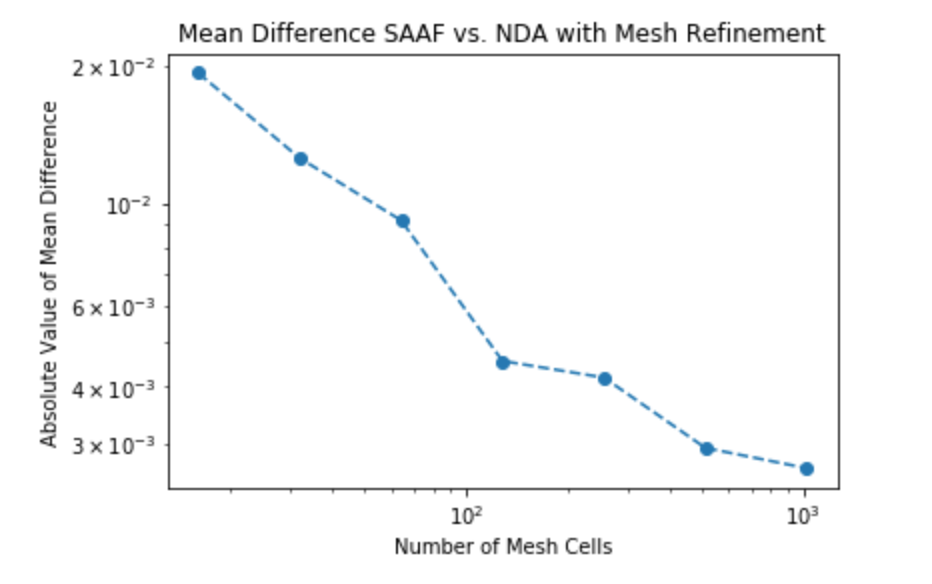
\includegraphics[width=.75\textwidth]{fig/NDAvsSAAF.png}
    \caption{SAAF/NDA Agreement with Mesh Refinement}
    \label{fig:SAAFvsNDA}
\end{figure}



Finally, we plot a 1-D line out of all three methods. For this problem we chose one test material with one group and some scattering. This is more of a gut check than a formal check of convergence. From this plot we can clearly see that NDA has provided a correction to diffusion, producing a solution that is much closer to the higher order equation than diffusion by itself. 

\begin{figure}[H]
    \centering
    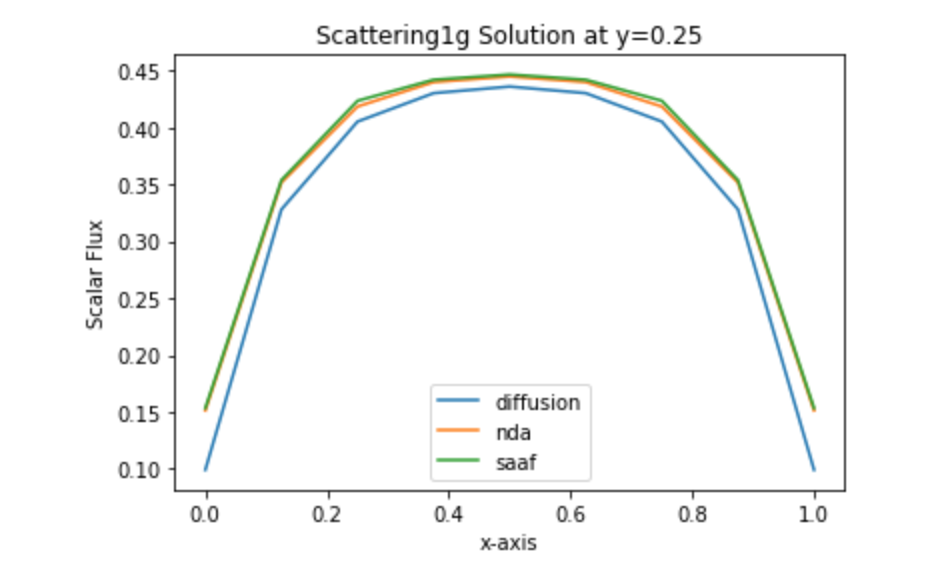
\includegraphics[width=.75\textwidth]{fig/LineOut25.png}
    \caption{Comparison of Diffusion, SAAF, and NDA}
    \label{fig:comparison}
\end{figure}

From the results of these three checks, we determine that we are in agreement with previously published work on SAAF+NDA and have implemented a working version. 

\chapter{Numerical Results}
\label{sec:results}
\section{One Material}
For the first test problem we used a single material with  upscattering throughout a 20 by 20 domain with a constant source. We used cross sections for the seven group moderator material in the C5G7 benchmark problem. \cite{C5G7}.  
% \subsection{Cross Sections}
% For experimentation purposes, we created a fake seven group material with significant upscattering. The scattering block is given below.
% \begin{table}
% \begin{center}
%     \begin{tabular}{|c|c|c|c|c|c|c|c|}
%     \hline
%     & g'=1 & g'=2 & g'=3 & g'=4 & g'=5 & g'=6 & g'=7  \\
%     \hline    
%     g = 1 & 10 & 1 & 1 & 1 & 0 & 0 & 0  \\
%     \hline    
%     g = 2 & 0 & 10 & 1 & 1 & 1 & 0 & 0  \\
%     \hline    
%     g = 3 & 0 & 0 & 10 & 1 & 1 & 1 & 0  \\
%     \hline    
%     g = 4 & 0 & 0 & 0 & 10 & 1 & 1 & 1  \\
%     \hline    
%     g = 5 & 0 & 0 & 0 & 1 & 10 & 1 & 1  \\
%     \hline    
%     g = 6 & 0 & 0 & 0 & 1 & 1 & 10 & 1  \\
%     \hline    
%     g = 7 & 0 & 0 & 0 & 1 & 1 & 1 & 10  \\
%     \hline
%     \end{tabular}
% \end{center}
% \caption{Scattering Matrix for Test Material}
% \end{table}
The problems were run on a single processor of a MacBook Pro. 
\begin{center}
    \begin{tabular}{|c|c|c|}
    \hline
    & Runtime (s) & GS Iterations \\
    \hline
    TG-NDA & 5465.00732 & 9 \\
    NDA & 14513.23 & 31 \\
    \hline
    \end{tabular}
\end{center}
The two-grid method provides a considerable acceleration of the Gauss-Seidel method. While when using TG-NDA each iteration takes slightly longer as the correction term must be calculated, it more than makes up for it with a considerable decrease in the number of iterations necessary to reach convergence. 
\section{Two Materials}
The second problem consists of two materials in a concentric geometry with a box source in the center. The first material, located in the center and outer layer, is the C5G7 moderator material used above and the second material has the same total cross sections and pattern of upscatter, but with higher absorption and lower total scattering. Both materials have seven groups. There is a box source in the center that emits 70\% in the highest energy group, 20\% in the second highest, and 10\% in the third.
\begin{figure}
    \centering
    
\includegraphics[width=.3\textwidth]{fig/Geometry.png}
    \caption{Geometry of Two-Material Test Problem}
    \label{fig:test_geometry}
\end{figure}

\begin{center}
    \begin{tabular}{|c|c|c|}
    \hline
    & Runtime (s) & GS Iterations \\
    \hline
    TG-NDA & 4221.92 & 8 \\
    NDA & 10381.52 & 25 \\
    \hline
    \end{tabular}
\end{center}

Again, TG-NDA showed a significant improvement over the unaccelerated Gauss Seidel, taking roughly a third of the number of iterations. 

\chapter{Conclusion \& Future Work}
\label{sec:future}

In this work we derived and implemented a two grid acceleration scheme for the nonlinear diffusion acceleration equations with neutron upscattering. In our tests problems, we observe a reduction in the number of Gauss-Seidel iterations necessary to resolve the upscattering of roughly a factor of three. The current implementation is in a lightweight code developed in python that is only designed as a proof of concept. We intend to implement a heavier-duty C++ version into the Slaybaugh Lab's neutron transport code, Bay Area Radiation Transport. With that implementation we can begin to test larger problems and understand how the method scales.

\section{Possible Extensions to TG-NDA}
There are a number of modifications to our implementation that could be interesting to explore with TG-NDA. 

\subsection{Other Discretization Schemes}
\subsubsection{$P_N$ angular discretization}
Our derivation is specific to the $S_N$ equations. It is possible to derive the higher order equation using $P_N$ instead \cite{zheng-thesis}. 
\subsubsection{Discontinuous Finite Elements}
In our implementation we use continuous finite elements to discretize in space. Discretizing NDA using discontinuous finite elements, as done in \cite{Schunert2016}, would change the form of TG-NDA. 
\subsection{Other Higher Order Equations}
We chose to pair NDA with SAAF, however other equations could be used as well, such as the even-parity equation \cite{Noh1996}.
\subsection{Applications to Criticality Problems}
In this work we only focused on fixed-source problems for shielding applications, however many materials commonly used in nuclear reactors, such as water, heavy water, or graphite, also exhibit significant upscattering. Performing criticality calculations using our method would be a straightforward extension involving only an additional later of iteration to perform the eigenvalue calculation. 

\begin{appendices}
  \chapter{FEM on an Unstructured Triangular Grid}
  \label{sec:spatial}
  \section{Continuous FEM on an Unstructured Grid}
To discretize in space we will be using the continuous finite element method with bilinear basis functions on an unstructured triangular mesh. The mesh is generated with the Triangle library \cite{shewchuk96b} via a Delaunay triangulation algorithm. 
\par
To integrate over the triangles, we have implemented a 2nd degree Gaussian Quadrature approximation over the standard triangle,
\begin{align}
    \iint_{T_{st}} f(\xi, \eta) d\xi d\eta \approx \frac{1}{6}\left [ f\left( 0, \frac{1}{2} \right ) + f \left( \frac{1}{2}, 0 \right) + f \left( \frac{1}{2}, \frac{1}{2} \right)\right].
\end{align}
We are working with an unstructured grid of triangles, so we must additionally map nodes on the standard triangle to an arbitrary element. This is done by the \texttt{gaussNodes()} function in this \texttt{FEGrid} class. 
\begin{figure}[h]
    \centering
    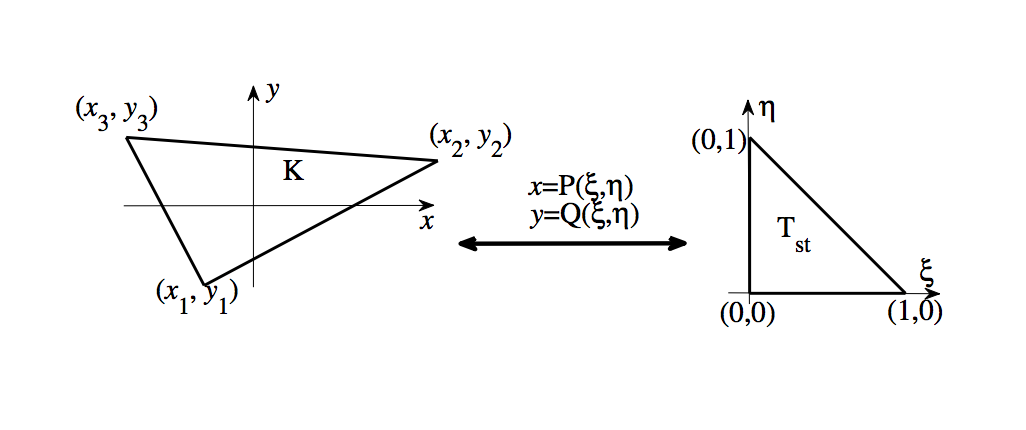
\includegraphics[width=0.75\textwidth]{fig/TriangleMapping}
    \caption{Linear mapping between an element K and the standard triangle}
    \label{fig:my_label}
\end{figure}
The mapping is given as follows
\begin{align}
    x &= P(\xi, \eta) = x_1 + \xi(x_2 - x_1) + \eta(x_3 - x_1) \\
    y &= Q(\xi, \eta) = y_1 + \xi(y_2 - y_1) + \eta(y_3 - y_1)
\end{align}
After applying the transformation we have,
\begin{align}
 \iint_{K} F(x, y) dx dy = \iint_{T_{st}}F(P(\xi, \eta), Q(\xi, \eta))|J(\xi, \eta)|d\xi d\eta
\end{align}
where $|J(\xi, \eta)|$ is the Jacobian of the transform which is equal to $2Area_K$. This gives the final quadrature rule as
\begin{align}
 \iint_{K} &F(x, y) dx dy = 2A_k\iint_{T_{st}}F(P(\xi, \eta), Q(\xi, \eta))d\xi d\eta \\
 &\approx \frac{1}{6}\left [ F\left( P(0), Q(\frac{1}{2}) \right) + F \left( P(\frac{1}{2}), Q(0) \right) + F \left( P(\frac{1}{2}), Q(\frac{1}{2}) \right)\right].
\end{align}

\section{Weak Form of NDA}
Similar to the higher order equation, we discretize  Eq. 4 via the continuous finite element method by multiplying by a test function and integrating over the domain. This gives the following weak form:

Find $\varphi_{d, g} \in W_D$ such that

  \begin{align}
  \left(D_\rg \nabla \varphi_\rg^{k+1/2}, \nabla \varphi^*_\rg\right)_\mathcal{D} &+ \left(\vec{\bf{D}_\rg}\varphi_\rg^{k+1/2} , \nabla \varphi^*_\rg\right)_\mathcal{D} +  \left(\sigma_{r,\rg} \varphi_{\rg}^{k+1/2}, \varphi^*_\rg\right)_\mathcal{D} = \nonumber \\
   \left(\sum\limits_{\substack{\rg'=1}}^\mm{g-1} \sigma_{\mm{s},\rg' \to\rg}\varphi_{\rg}^{k+1/2}, \varphi^*_\rg\right)_\mathcal{D} &+ \left(\sum\limits_{\substack{\rg'=\rg+1}}^\mm{G} \sigma_{\mm{s},\rg' \to\rg}\varphi_{\rg}^{k}, \varphi^*_\rg\right)_\mathcal{D} 
  + \left(S_\mathrm{f,g}, \varphi^*_\rg\right)_\mathcal{D}  \label{k1/2}
  \end{align}


The error (Eq. 8) is similarly discretized via CFEM.
  \begin{align}
  \left(\left< D\xi \right >\nabla \varphi_{\epsilon}^{k+1}, \nabla \varphi^* \right)_\mathcal{D} + \left(\left<\vec{\bf{D}\xi} \right>\varphi_{\epsilon}^{k+1}, \nabla \varphi^* \right)_\mathcal{D} &+ \left(\left<\sigma_r \right>\phi_{\epsilon}^{k+1}, \varphi^* \right)_\mathcal{D}  \nonumber \\= \left(\left<R^{k+1} \right>, \varphi^* \right)_\mathcal{D} &+ \left(\left<S_\mathrm{f,g} \right>, \varphi^* \right)_\mathcal{D} 
  \end{align}

\section{Weak Form of the Higher Order Equation}
We apply a finite element discretization to the higher order equation, SAAF, by first multiplying Eq. \ref{eq:SAAF} by a test function $\psi*$ and integrating over the domain $D$.

\begin{equation}
    \left ( -\vec{\Omega} \cdot \vec{\nabla}\frac{1}{\sigma_t}\vec{\Omega} \cdot \vec{\nabla} \psi, \psi* \right )_D + \left ( \sigma_t \psi, \psi* \right )_D = \left ( Q, \psi* \right)_D - \left ( \vec{\Omega} \cdot \vec{\nabla}\frac{Q}{\sigma_t}, \psi* \right)_D
\end{equation}
Integrating by parts,

\begin{align*}
        \left ( \vec{\Omega}\frac{1}{\sigma_t}\vec{\Omega}\cdot \vec{\nabla}\psi, \vec{\nabla}\psi* \right)_D &-     \left ( \vec{\Omega}\cdot \hat{n} \frac{1}{\sigma_t}\vec{\Omega} \cdot \vec{\nabla} \psi,\psi* \right)_{\Gamma} + \left ( \sigma_t \psi, \psi* \right )_D = \\
        \left ( Q, \psi* \right)_D &+ \left ( \vec{\Omega} \frac{Q}{\sigma_t}, \vec{\nabla}\psi* \right)_D - \left ( \vec{\Omega}\cdot \hat{n} \frac{Q}{\sigma_t}, \psi* \right)_{\Gamma} 
\end{align*}


\end{appendices}

\bibliography{mybibfile.bib}
\bibliographystyle{plain}
\end{document}
